% !TEX root = IROS2020.tex


\section{Simulation Results}
\label{sec:simulation}
\subsection{ Implementation of Algorithms for $\mathbf{H}_{GN}$ and $\mathbf{J}$}
%First, We obtain the derivative of dynamic equation $\frac{\partial \mathbf{f}}{\partial \mathbf{x}}$, $\frac{\partial \mathbf{f}}{\partial \mathbf{u}}$ using an automatic differentiation (AD) package. Among many AD packages, CasAdi~\cite{andersson2019casadi} is selected as it provides a symbolic framework that are easily integrated with MATLAB\textsuperscript{\textregistered} as well as supports the generation of self-contained C-code. Using this generated C-code for $\frac{\partial \mathbf{f}}{\partial \mathbf{x}}$, $\frac{\partial \mathbf{f}}{\partial \mathbf{u}}$, 

Algorithm~\ref{alg:GNHA} and Algorithm~\ref{alg:AG} are implemented in C-language for their fast computation. Evaluations of $\frac{\partial \mathbf{f}}{\partial \mathbf{x}}$, $\frac{\partial \mathbf{f}}{\partial \mathbf{u}}$ are also included in the C-code. The $\mathbf{f}$ is chosen as a discretized cart-pole dynamics equation.
We compare their computation time to that of $\mathbf{H}_{GN}$ auto-generated by CppAD~\cite{bell2012cppad} along with CppADCodeGen. Using CppAD, we obtain the symbolic expression of $\boldsymbol{\phi}_i$ by propagating controls $\mathbf{u}_i$ and initial states through~\eqref{eq:states_i}, and obtain $\frac{\partial \boldsymbol{\phi}_i}{\partial \mathbf{U}_N}$ via automatic differentiation. Lastly, using~\eqref{eq:H_GN1}, $\mathbf{H}_{GN}$ are constructed. Matrix operations are handled by Eigen 3 library~\cite{eigenweb}. 
Also, comparison with $\mathcal{O}(N^3)$ algorithm written in C is made.  As shown in Figure~\eqref{fig:H_O2O3}, our proposed algorithm outperforms the other methods for $N\geq20$ and its performance becomes better as $N$ increases. %Table~\ref{tab:elapsedtime} demonstrates 
Figure~\ref{fig:H_O2O3_bar} displays the breakdown of solve time for the cart-pole system. Using the inefficient $\mathcal{O}(N^3)$ algorithm, the calculation of  $\mathbf{H}_{GN}$ and $\mathbf{J}$ took more than half of the total solve time while it is significantly decreased with the proposed algorithm. 

\begin{figure}
	\centering
	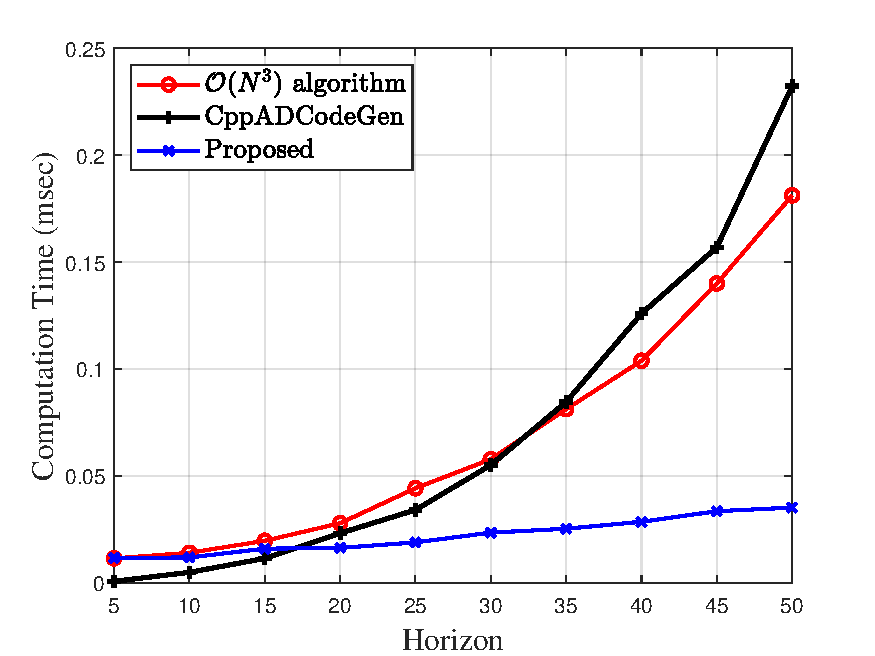
\includegraphics[width=0.8\columnwidth]{Figures/O2O3.pdf}
	\caption{Comparison of calculation times of the algorithms for Gauss-Newton Hessian approximaion with respect to the length of the Horizon.}
	\label{fig:H_O2O3}
\end{figure}


%\begin{table}
	
%	\center
	
%	\begin{tabular}{cccccc}
		
%		\hline
		
%		System & $N=20$ & $N=30$ & $N=40$ & $N=50$\\\hline
		
%		Car Parking  &  $35.4 ~\rm{sec}$ & $123.7 ~\rm{sec}$ & $351.6 ~\rm{sec}$ & $889.4 ~\rm{sec}$\\
		
%		Cart-Pole &  $59.7 ~\rm{sec}$ & $292.0 ~\rm{sec}$ & $1038.1 ~\rm{sec}$ & $2471.3 ~\rm{sec}$
		
%		\\ \hline
		
%	\end{tabular}
%	\vspace{2px}
%	\caption{Elapsed time in generation and building of a library file for $\frac{\partial \boldsymbol{\Phi}}{\partial \mathbf{U}_N}$ using CppADCodeGen.  }
%	\label{tab:elapsedtime}
%\end{table}


%\begin{table}
	
%	\center
	
%	\begin{tabular}{cccc}
		
%		\hline
		
%		System & Proposed & iLQG & ALTRO\\\hline
		
%		Car Parking ($N=100$)  &  $3.1041 (15)$ & $4.7082 (132)$ &  \\
		
%		Cart-Pole ($N=50$) &  $3597 (24)$ & $3597 (30)$ &  
		
%		\\ \hline
		
%	\end{tabular}
%	\vspace{2px}

%	\caption{The value of the objective and iteration number at the termination of algorithms. }
%	\label{tab:complexity}
%\end{table}



\subsection{Trajectory Optimization}
We tested the proposed algorithm for the trajectory optimization of different dynamic systems. Each optimization problem uses a quadratic objective and inequality constraints with upper and lower bounds on control inputs. Simulation is performed on a desktop computer with an Intel\textsuperscript{\textregistered} i7-8700 CPU running at 3.2 GHz and 32GB RAM. For performance comparison, each trajectory optimization problem is solved with SNOPT~\cite{gill2002snopt}, IPOPT~\cite{wachter2006implementation}, iLQG~\cite{6907001}, and the proposed algorithm. For SNOPT and IPOPT, functions that compute cost, analytical gradient, and constraints are written in C. The software package of iLQG is obtained from~\cite{iLQG2015}, and we converted it into a C-code for fair comparison of solve time. 
 %To compare Gauss-Newton Hessian approximation to different Hessian approximation using quasi-Newton methods, we also included Broyden–Fletcher–Goldfarb–Shanno (BFGS) algorithm~\cite{fletcher2013practical}. 
The following is a list of dynamic systems for benchmark.

\subsubsection{Cartpole} The system must perform a swing-up maneuver from randomly generated initial states while respecting control limits.

%\begin{figure}
%	\centering
%	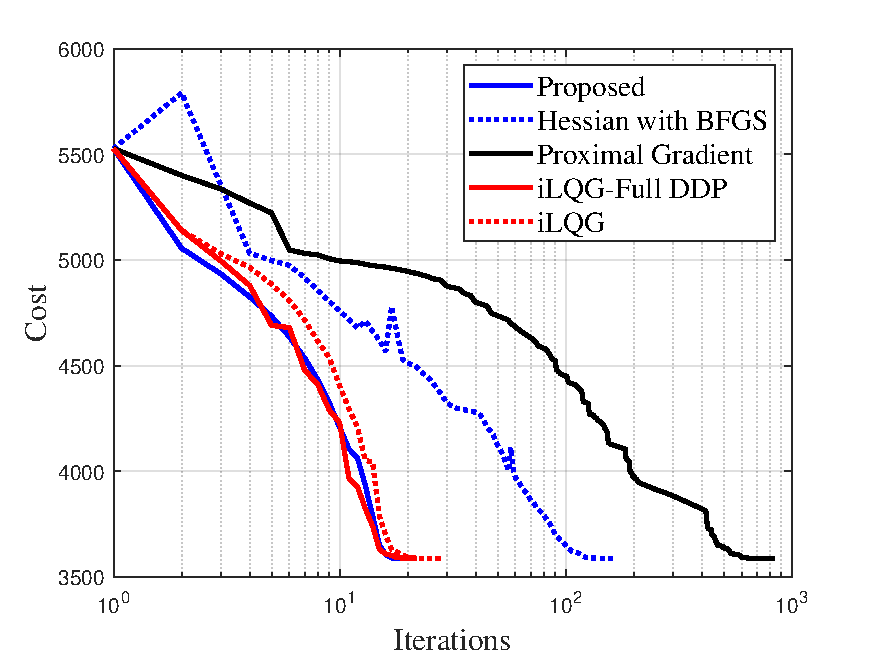
\includegraphics[width=\columnwidth]{Figures/Iteration_cartpole.pdf}
%	\caption{Cart-Pole system with $N=50$}
%	\label{fig:IT_CARTPOLE}
%\end{figure}
%\begin{figure}
%	\centering
%	\includegraphics[width=\columnwidth]{Figures/Iteration_carpark.pdf}
%	\caption{Car parking problem with $N=100$}
%	\label{fig:It_CARPARK}
%\end{figure}


%\begin{figure}
%	\centering
%	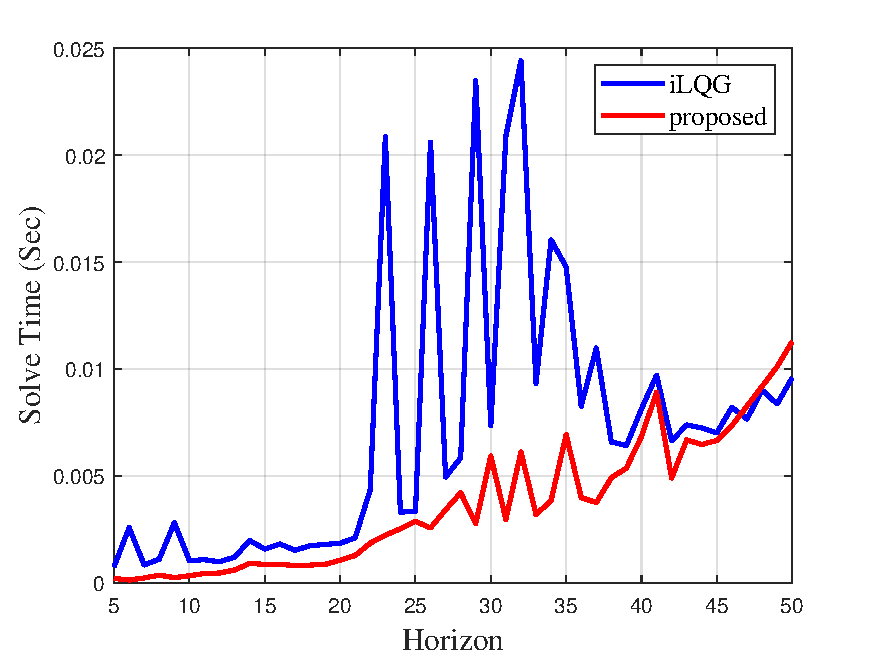
\includegraphics[width=0.8\columnwidth]{Figures/Cart_Pole_Solvetime.pdf}
%	\caption{Comparison of solve time of Cart-Pole System with respect to the Horizon Length.}
%	\label{fig:H_CARTPOLE}
%\end{figure}

\begin{figure}
	\centering
	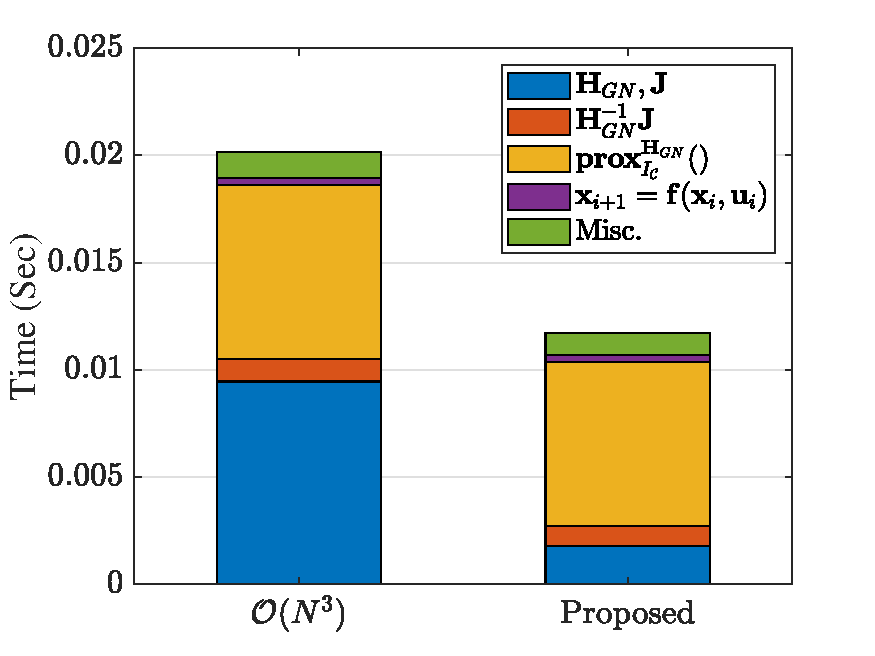
\includegraphics[width=0.7\columnwidth]{Figures/O2O3_bar.pdf}
	\caption{Breakdown of solve time for the cart-pole system with $N=50$. $\mathbf{H}_{GN}, \mathbf{J}$ are calculated with $\mathcal{O}(N^3)$ algorithm on the left and the proposed $\mathcal{O}(N^2)$ algorithm on the right. The blue area indicates required time for calculation of $\mathbf{H}_{GN}, \mathbf{J}$. }
	\label{fig:H_O2O3_bar}
\end{figure}


\begin{figure}
	\centering
\begin{subfigure}[b]{1.0\columnwidth}
	\centering
	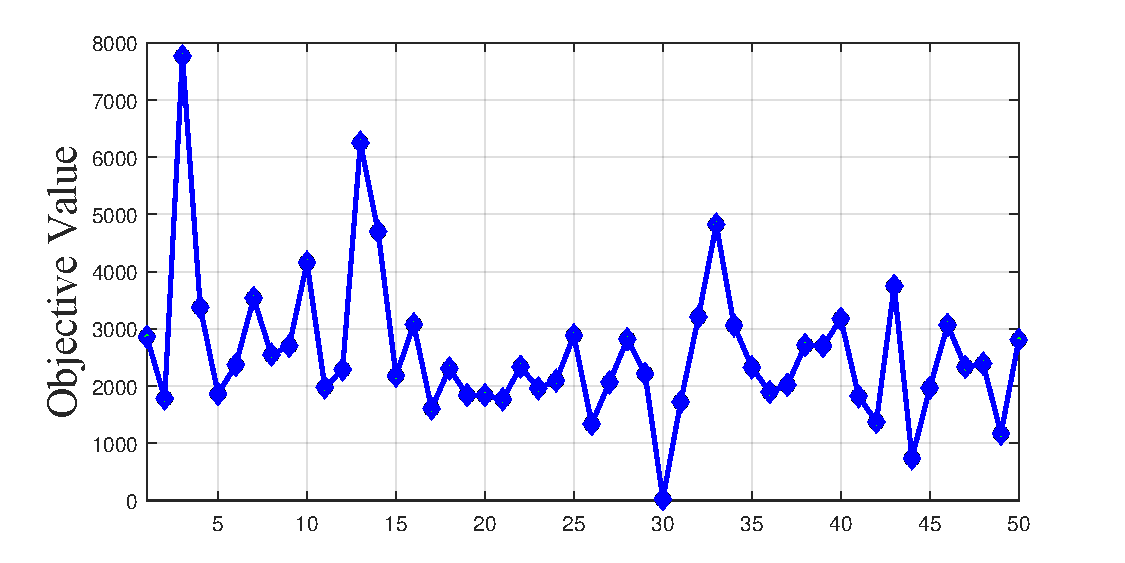
\includegraphics[width=0.9\columnwidth]{Figures/cartpole_cost_comparison10.pdf}\vskip -0.5em
	\caption{{$N=10$}}
\end{subfigure}\vskip -0.2em
\begin{subfigure}[b]{1.0\columnwidth}
	\centering
	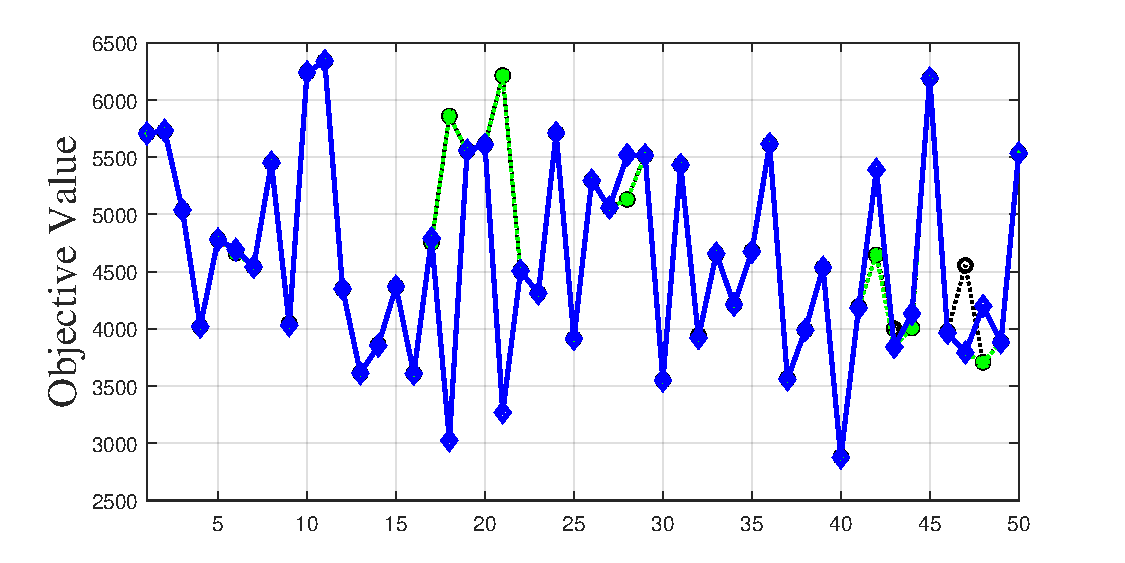
\includegraphics[width=0.9\columnwidth]{Figures/cartpole_cost_comparison50.pdf}\vskip -0.5em
	\caption{{$N=50$}}	
\end{subfigure}	\vskip -0.2em	
	\centering
	\begin{subfigure}[b]{1.0\columnwidth}
	\centering
	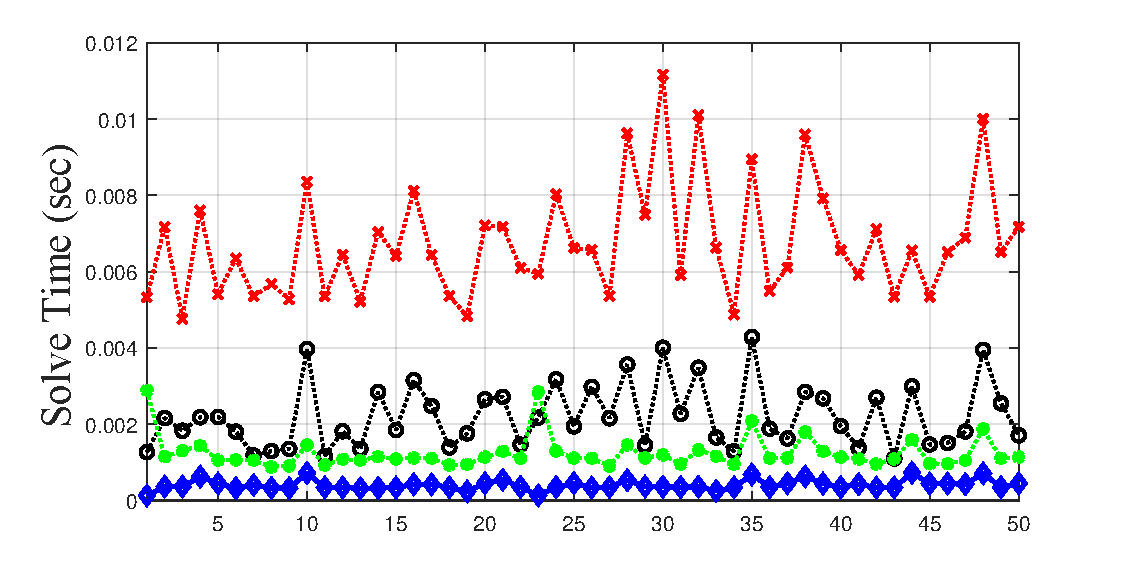
\includegraphics[width=0.9\columnwidth]{Figures/cartpole_time_comparison10.pdf}\vskip -0.5em
	\caption{{$N=10$}}	
	\end{subfigure}\vskip -0.2em
	\begin{subfigure}[b]{1.0\columnwidth}
	\centering
	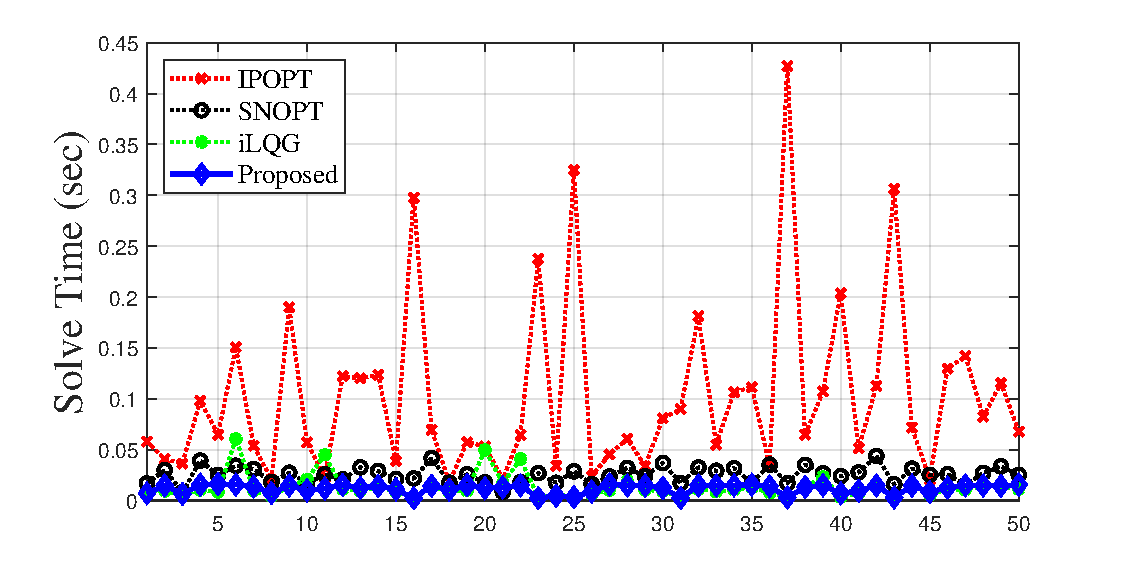
\includegraphics[width=0.9\columnwidth]{Figures/cartpole_time_comparison50.pdf}\vskip -0.5em
	\caption{{$N=50$}}	
	\end{subfigure}	\vskip -0.2em	
	\caption{Objective values and solve time  of the cart-pole system with different horizons. Each figure presents 50 problem instances with randomly generated initial states. }
	\label{fig:Car_Parking_comparison}
\end{figure}

\begin{figure}
	\centering
	\begin{subfigure}[b]{1.0\columnwidth}
		\centering
		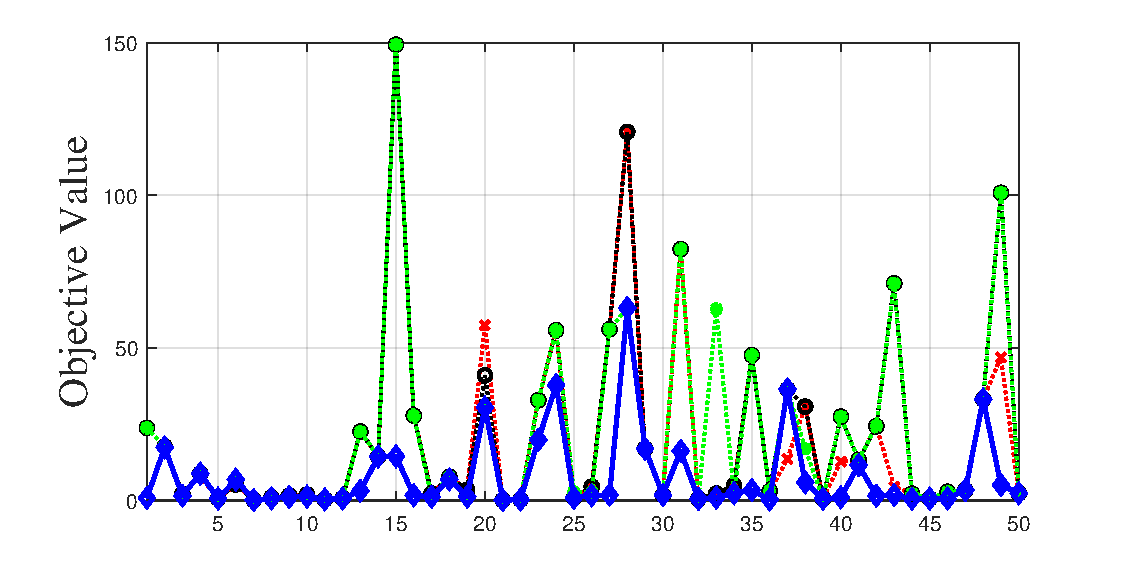
\includegraphics[width=0.9\columnwidth]{Figures/Car_Parking_cost_comparison50.pdf}\vskip -0.5em
	\caption{{$N=50$}}
	\end{subfigure}\vskip -0.2em
	\begin{subfigure}[b]{1.0\columnwidth}
		\centering
		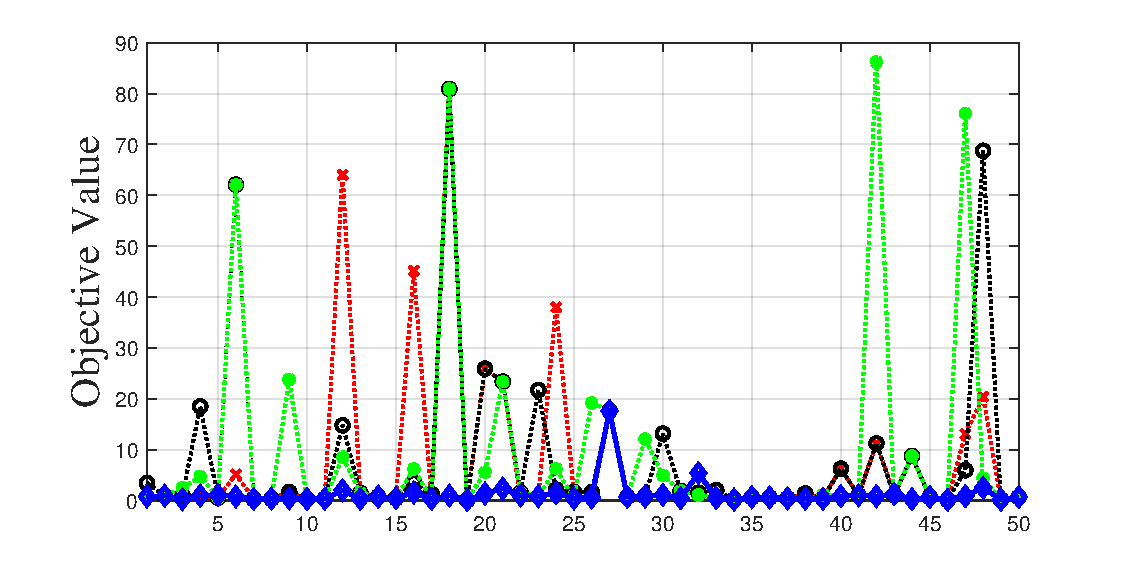
\includegraphics[width=0.9\columnwidth]{Figures/Car_Parking_cost_comparison100.pdf}\vskip -0.5em
	\caption{{$N=100$}}
	\end{subfigure}		
	\centering\vskip -0.2em
	\begin{subfigure}[b]{1.0\columnwidth}
		\centering
		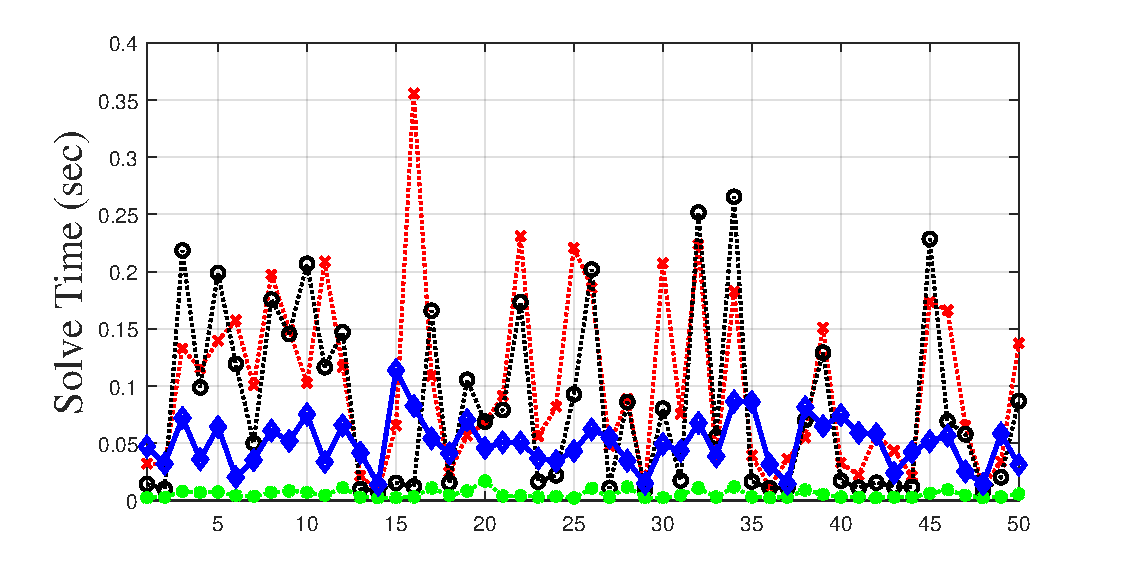
\includegraphics[width=0.9\columnwidth]{Figures/Car_Parking_time_comparison50.pdf}\vskip -0.5em
	\caption{{$N=50$}}	\end{subfigure}\vskip -0.2em
	\begin{subfigure}[b]{1.0\columnwidth}
		\centering
		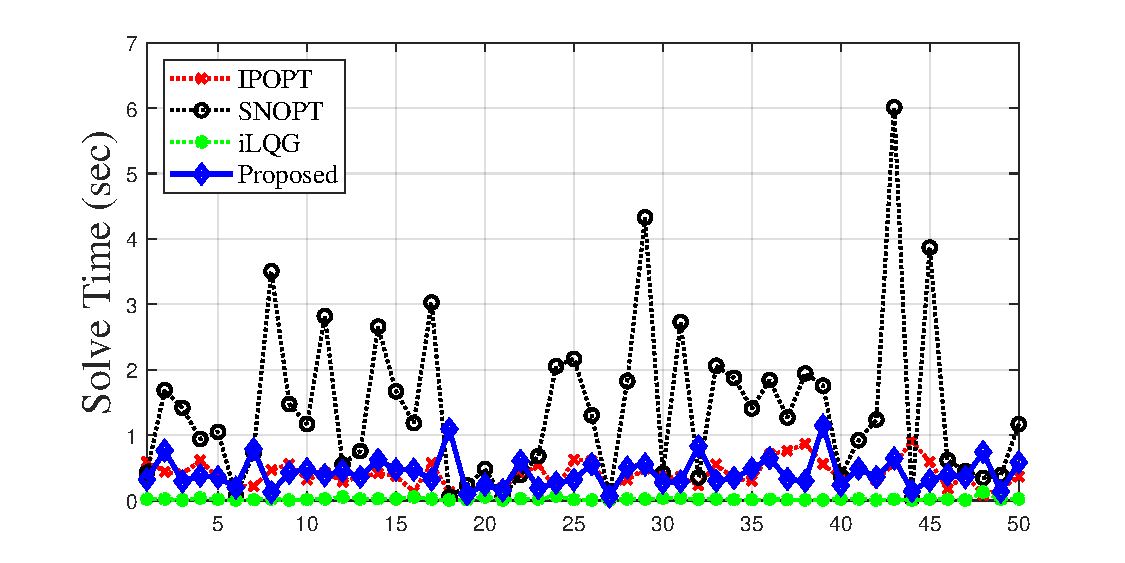
\includegraphics[width=0.9\columnwidth]{Figures/Car_Parking_time_comparison100.pdf}\vskip -0.5em
	\caption{{$N=100$}}	\end{subfigure}	\vskip -0.2em	
	\caption{Objective values and solve time of the car parking problem with different horizons. Each figure presents 50 problem instances with randomly generated initial states. }
	\label{fig:cartpole_comparison}
\end{figure}

\begin{figure}
	\centering
\vspace{-1em}
	\begin{subfigure}[b]{0.9\columnwidth}
		\centering
		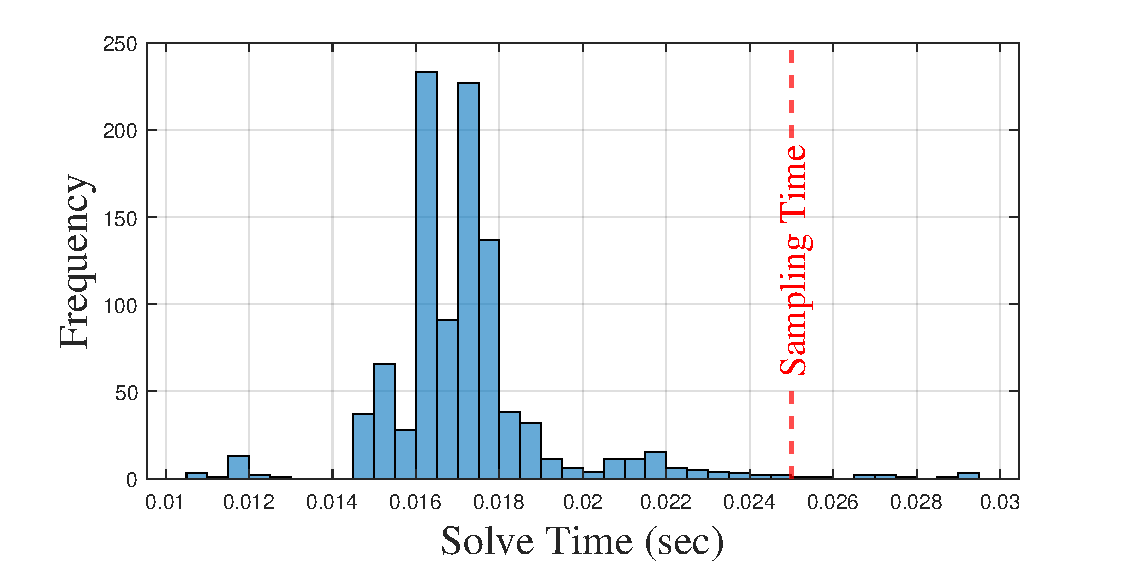
\includegraphics[width=1.0\columnwidth]{Figures/Solve_Time_Histogram_12.pdf}
	\end{subfigure}
\vskip -0.5em
	\begin{subfigure}[b]{0.9\columnwidth}
		\centering
		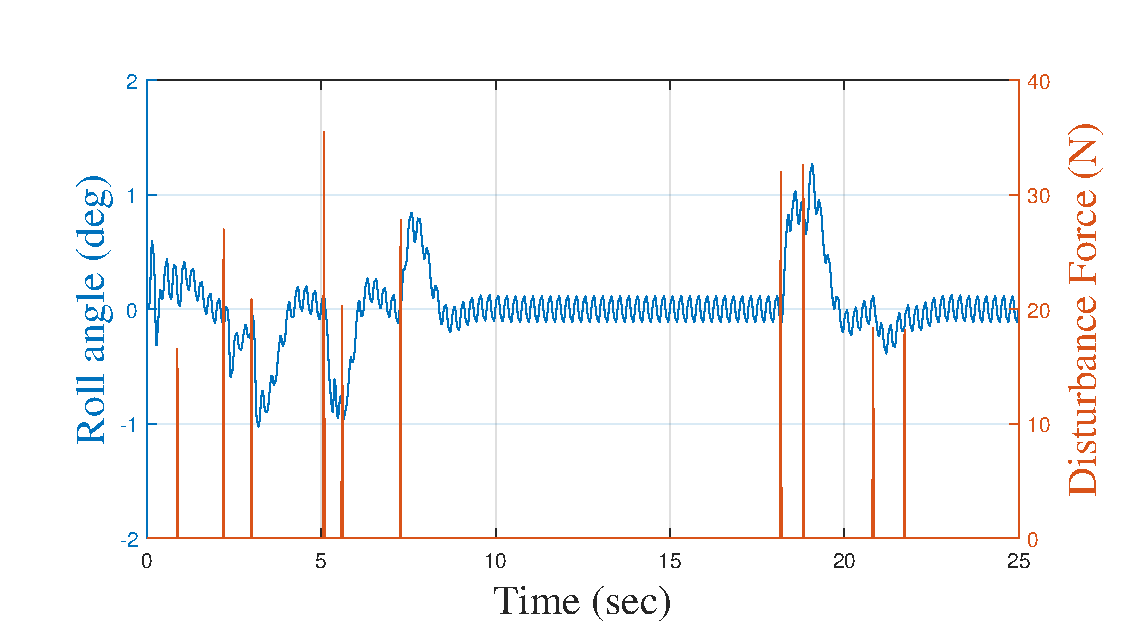
\includegraphics[width=1.0\columnwidth]{Figures/Roll_Angle_Disturbance_Force_12.pdf}
	\end{subfigure}		
	\caption{Nonlinear Model Predictive Control of a quadrupedal trotting with the speed of $1.5~\rm{m/sec}$. Random disturbance forces are applied, and their magnitude are shown in the bottom figure. Top figure displays histogram of MPC solve time during simulation.  }
	\label{fig:quadruped}
\end{figure}
%\subsubsection{Acrobat and Pendubot}
	%\vspace{-10em}

%Both are under-actuated double pendulum systems. Acrobat is limited to actuation at the “elbow” joint while Pendubot is limited to actuation at the "shoulder" joint. Both are tasked with swinging upright from the downward position.

\subsubsection{Car Parking}

The system has four states with $(x,y,\theta,v)$ where $x,y$ is the position of the car, $\theta$ is the orientation of the car, and $v$ is the velocity of the front wheels~\cite{6907001}. The two control inputs are $\omega$ the front wheel angle and $a$ the front wheel acceleration. Initially, the car is placed at random states and has to reach a desired state of $(0,0,0,0)$ at the end of the Horizon ($N=100$). 

Figure~\ref{fig:Car_Parking_comparison} shows objective values and solve time of the cart-pole system at the termination of the algorithms. In all the cases with $N=10$, the proposed algorithm provides the shortest solve time while objective values converged to the same value across the algorithms. With the larger value of $N=50$, the proposed algorithm yields on average the best objective value. However, the solve time is similar to that of iLQG.

The results of the car parking scenario are shown in Figure~\ref{fig:cartpole_comparison}. Clearly, the proposed algorithm displays the best performance in terms of the objective value significantly surpassing the other algorithms. The iLQG has the shortest solve time, but the algorithm provides values that are very far from the best ones for many cases. SNOPT and IPOPT provide objective values similar to iLQG in spite of long solve time.   


\subsection{Nonlinear Model Predictive Control}

%\subsubsection{Cartpole}

Nonlinear MPC control of a quadrupedal robot is demonstrated to validate proposed algorithm's capability to handle systems with a large number of states and control inputs. The system is modeled as a 6 DoF floating-rigid body controlled by 3 dimensional ground reaction forces at 4 legs, constituting 12 control inputs in total. This model serves as a simplified model of quadrupeds for control design and trajectory generation~\cite{8594448,8283570}. Linearized friction cone constraints are imposed on ground reaction forces as linear inequality constraints and gait sequence for the timing of stance and swing legs is imposed with equality constraints that ground reaction forces of the airborne legs should be equal to zero. The length of horizon is selected as $N=12$ with a sampling time of $0.025~\rm{sec}$. The result of trotting gait with the forward velocity of $1.5~\rm{m/sec}$ is shown in Figure~\ref{fig:quadruped}. Other types of gait such as galloping, bounding, pacing also can be controlled while handling push disturbances~\footnote{\label{note1}These results are only shown in the submitted video due to the maximum page limit}. Note that this system cannot be controlled by control-limited iLQG because of the linearized friction cone constraints.

In addition to nonlinear MPC of a quadrupedal robot, we tested our algorithm for nonlinear MPC of cart-pole, pendubot (only actuation at the "shoulder" joint), and acrobat (only actuation at the "elbow" joint) systems which are examples of nonlinear under-actuated systems~\footnoteref{note1}. 


\section{Discussion and Future Works}
\subsection{Nonlinear Constraints}
Extension of the proposed algorithm can be easily made to include more general inequality constraints although only linear inequalities are addressed in the current form of the proposed framework. Without changing the main algorithm to find $\delta \mathbf{U}$, only the proximal operator using QP solver can be replaced with the one using more general solvers such as nonlinear programming solvers to handle nonlinear constraints. This is possible due to modular structure of the proposed framework where calculation of search direction and handling of inequality constraints are carried out separately,     


\subsection{State Constraints}
Modification can be easily made to extend the proposed algorithm's functionality to handle state or mixed state-input constraints. One possible modification can come from augmented Lagrangian method that changes the objective function to the Lagrangian with additional quadratic penalty terms, and iteratively updates Lagrangian multipliers and penalty weights until convergence. %This AL method is widely used in constrained optimal control problems. For example, in~\cite{howell2019altro}, the AL method is used to propose a fast solver for constrained trajectory optimization, and the work in\cite{lantoine2012hybrid} utilizes the AL method to propose hybrid differential dynamic programming algorithm for constrained optimal control problems. 
 As application of the AL method will only change the objective function to the augmented Lagrangian without directly adding state or mixed constraints to the formulation, we predict that this modification can be done without major changes of the framework.      
\subsection{Long-Term Horizon MPC Problem}
For a long horizon MPC problem, the proposed algorithm can be numerically costly as Algorithm~\ref{alg:GNHA} has computational complexity of $\mathcal{O}(N^2)$. % and this is briefly shown in the cart-pole system when $N>47$ in Figure~\ref{fig:IT_CARTPOLE}. 
%The main reason for low numerical efficiency is caused by the process to obtain the line search direction in~\eqref{eq:GNsearchdirection} as it involves  solving QP with a large dense matrix $\mathbf{H}_{GN}$. 
 One efficient approach to find the solution of~\eqref{eq:linopt} is the iterative LQR in~\cite{1469949} utilizing discrete-time Riccati equation which has $\mathcal{O}(N)$ computational complexity. However, since this approach does not provide Gauss-Newton Hessian Approximation matrix, we have to use unscaled version of the proximal operator which could decrease the rate of convergence resulting in more iterations. %This is briefly captured in a large number of iterations of Proximal Gradient algorithm in Figure~\ref{fig:IT_CARTPOLE} and~\ref{fig:It_CARPARK}.
Therefore, there should exist a lower range of $N$ that is favorable to the proposed algorithm, and vice versa.   
	%In order to perceive information about its surrounding environment, the quadruped was outfitted with a Hokuyo UTM-30LX-EW laser range finder as shown in Fig.~\ref{fig:architecture}. This sensor provides distance data in its scan plane with an angular resolution of $0.25^\circ$. To minimize the scan time, data was collected in the sagittal plane only for angles between $45^\circ$ above the horizontal, to $90^\circ$ below the horizontal, as shown in Fig.~\ref{fig:lidarscan}. It was assumed that the motion of the robot during the scan time of $12.5$ ms had a negligible effect on the data. Pitch correction from the IMU was used to rotate this data into global coordinates.
	
	%Following each scan, a simple line segmentation algorithm was applied to detect the ground plane and the front face of the obstacle. Nguyen et al. \cite{Siegwart07} provide a thorough overview of line segmentation algorithms for planar data, and report on the promising accuracy and processing speed of the Split and Merge algorithm \cite{Horowitz74}.  In order to further decrease the computational overhead of the algorithm, a simplification of the Split and Merge algorithm, the Iterative-end-point-fit (IEPF) algorithm \cite{Ramer72} was used here.  This algorithm begins by constructing a line between the first and last points of the data. It then proceeds to take the point furtherest from the line, splits the data into two halves about this point,  and reapplies the algorithm to each half. This recursive process is repeated until all data is within a threshold distance to any segment.
	
	%To  decrease the size of the input to the IEPF algorithm, data was first preprocessed to extract a contiguous subset of points that contained the ground plane. Starting at $90^\circ$ below the horizontal, the radial distance of successive data points was monitored for a large jump above a given threshold. All data after the first jump was discarded. In addition, $(x,z)$ data in the sagittal plane within a small tolerance was clustered together and averaged to further decrease the input size. Figure \ref{fig:lidarscan} shows the preprocessed data passed to IEPF, as well as its segmented output. The long first segment in this data represents the ground plane, while the second segment represents the front face of the obstacle. 
%The distance to the second segment $d_0$ and its length  $h_0$ were then used to provide a sensed obstacle distance and height to the approach adjustment and trajectory optimization algorithms. 
%This method was found to be effective during bounding at ~3Hz despite significant pitch and small roll oscillations which perturbed the lidar scan plane, as demonstrated further in Sec.\ref{sec:results}.

%\cite{Siegwart07} - Review\\
%\cite{Ramer72} - Iterative- End-Point-Fit \\
%\cite{Horowitz74} - Split and Merge

%\begin{figure}
%\center
%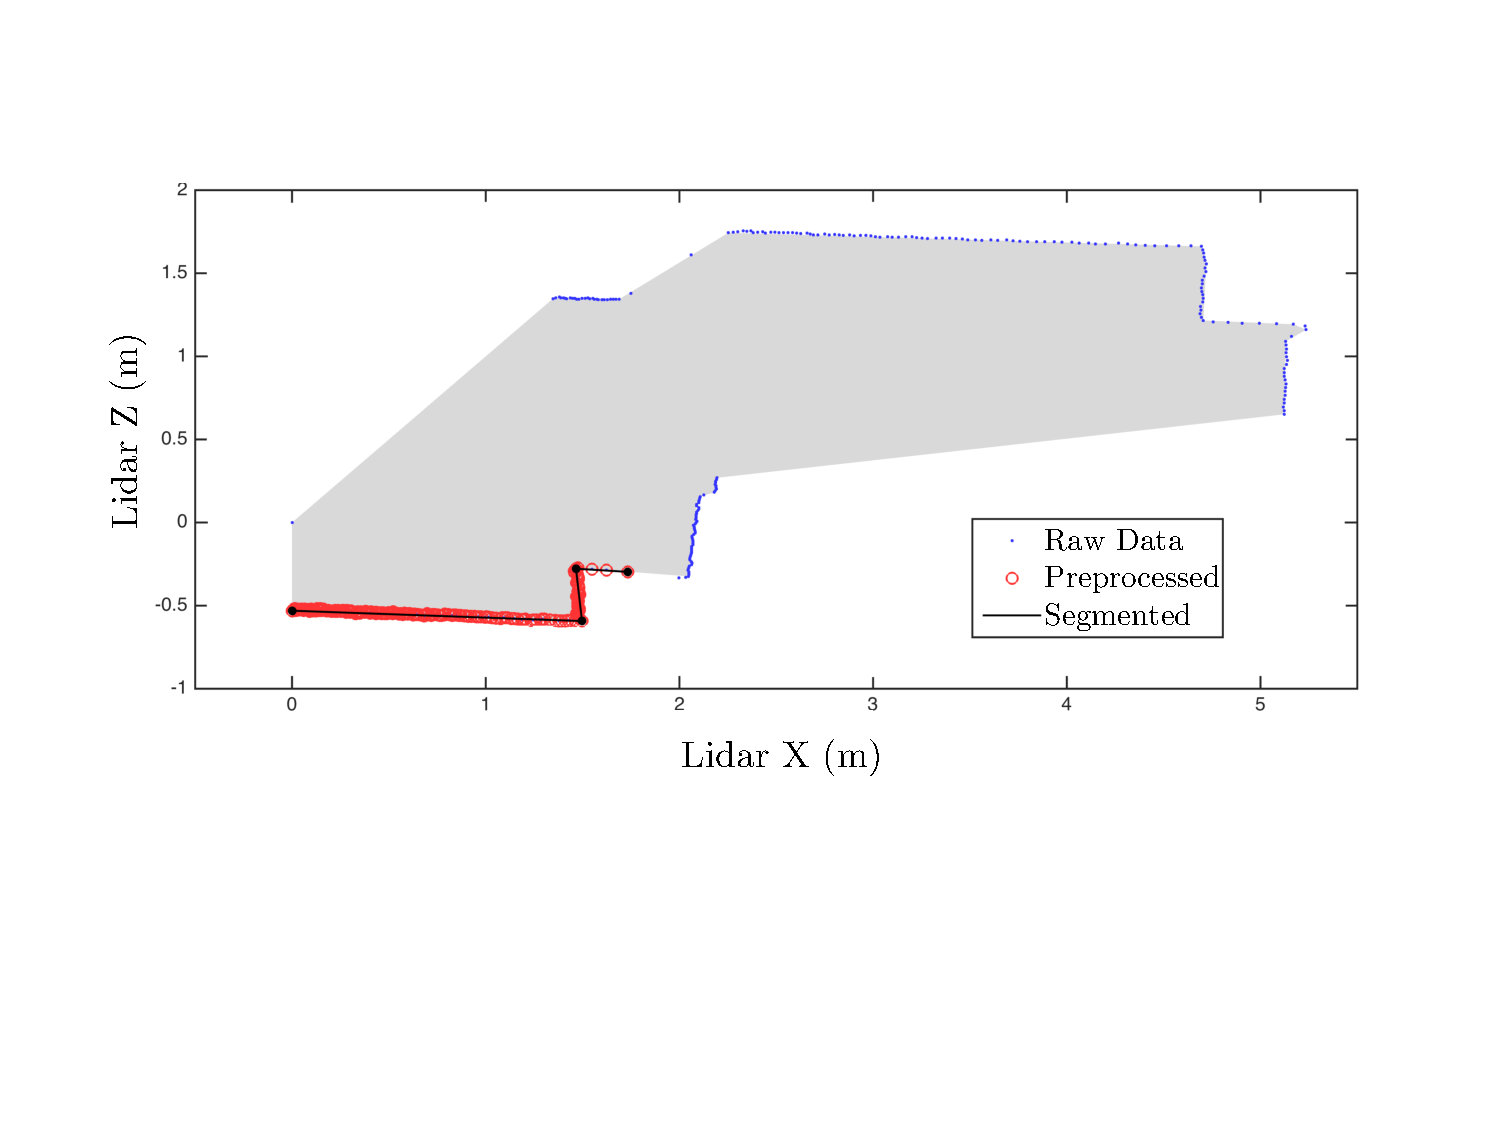
\includegraphics[width=.95\columnwidth]{Figures/HokData.pdf}
%\caption{Lidar data, preprocessing, and final segmentation for a characteristic scan over $135^\circ$ in the sagittal plane.}
%\label{fig:lidarscan}
%\end{figure}
